\documentclass[a4paper, 12pt, twoside]{article}
\usepackage[utf8]{inputenc}		% LaTeX, comprend les accents !
\usepackage[T1]{fontenc}		
\usepackage[francais]{babel}
\usepackage{lmodern}
\usepackage{ae,aecompl}
\usepackage[top=2.5cm, bottom=2cm, 
			left=3cm, right=2.5cm,
			headheight=15pt]{geometry}
\usepackage{graphicx}
\usepackage{eso-pic}	% Nécessaire pour mettre des images en arrière plan
\usepackage{array} 
\usepackage{hyperref}
\usepackage{pdfpages} % Package pour inclure des pages PDF
\usepackage{float}

%%%%%%%%%%%%%%%%%%%%%%%%%%%%%%%%%%%%%%%%
%    Page de garde (Pagedegarde.tex)   %
%%%%%%%%%%%%%%%%%%%%%%%%%%%%%%%%%%%%%%%%
% KAN Kevin, 2024

\makeatletter
\def\@ecole{Université Paris Nanterre}
\newcommand{\ecole}[1]{
  \def\@ecole{#1}
}

\def\@entreprise{Nom de l'entreprise}
\newcommand{\entreprise}[1]{
  \def\@entreprise{#1}
}

\def\@{\today}
\newcommand{\datedebut}[1]{
  \def\@datedebut{#1}
}


\def\@datefin{\today}
\newcommand{\datefin}[1]{
  \def\@datefin{#1}
}



\def\@specialite{Spécialité}
\newcommand{\specialite}[1]{
  \def\@specialite{#1}
}

\def\@ED{\'{E}cole Doctorale}
\newcommand{\ED}[1]{
  \def\@ED{#1}
}

\def\@doctorat{Doctorat}
\newcommand{\doctorat}[1]{
  \def\@doctorat{#1}
}

\def\@adresse{Adresse}
\newcommand{\adresse}[1]{
  \def\@adresse{#1}
}

\def\@directeur{directeur}
\newcommand{\directeur}[1]{
  \def\@directeur{#1}
}

\def\@encadrant{encadrant}
\newcommand{\encadrant}[1]{
  \def\@encadrant{#1}
}
\def\@membrea{Membre}
\newcommand{\membrea}[1]{
  \def\@membrea{#1\\}
}
\def\@membreb{Membre}
\newcommand{\membreb}[1]{
  \def\@membreb{#1\\}
}
\def\@membrec{Membre}
\newcommand{\membrec}[1]{
  \def\@membrec{#1\\}
}
\def\@membred{Membre}
\newcommand{\membred}[1]{
  \def\@membred{#1\\}
}
\def\@membree{Membre}
\newcommand{\membree}[1]{
  \def\@membree{#1\\}
}





\def\@juryb{}{}{}
\newcommand{\juryb}[3]{
  \def\@juryb{#1,	& #2	& #3\\}
}
\def\@juryc{}{}{}
\newcommand{\juryc}[3]{
  \def\@juryc{#1,	& #2	& #3\\}
}
\def\@juryd{}{}{}
\newcommand{\juryd}[3]{
  \def\@juryd{#1,	& #2	& #3\\}
}
\def\@jurye{}{}{}
\newcommand{\jurye}[3]{
  \def\@jurye{#1,	& #2	& #3\\}
}
\def\@juryf{}{}{}
\newcommand{\juryf}[3]{
  \def\@juryf{#1,	& #2	& #3\\}
}
\def\@juryg{}{}{}
\newcommand{\juryg}[3]{
  \def\@juryg{#1,	& #2	& #3\\}
}
\def\@juryh{}{}{}
\newcommand{\juryh}[3]{
  \def\@juryh{#1,	& #2	& #3\\}
}
\def\@juryi{}{}{}
\newcommand{\juryi}[3]{
  \def\@juryi{#1,	& #2	& #3\\}
}
\makeatother

\newcommand\BackgroundPic{%
	\put(0,0){%
		\parbox[b][\paperheight]{\paperwidth}{%
			\includegraphics[height=0.45\paperheight]{bordure.png}%
			\vfill
		}
	}
}
\newcommand\EtiquetteThese{%
	\put(0,0){%
		\parbox[t][\paperheight]{\paperwidth}{%
			\hfill
			%\colorbox{blue}{		
				\begin{minipage}[b]{2em}
					\includegraphics[width=4.0\textwidth]{logo_miage.png}\\					
					%\centering\Huge\textcolor{white}{M\\I\\A\\G\\E\\}
					\vspace{0.2cm}
				\end{minipage}
			%}
		}
	}
}

\makeatletter
\newcommand{\pagedegarde}{
\newgeometry{top=2.5cm, bottom=1cm, left=2cm, right=1cm}
\AddToShipoutPicture*{\BackgroundPic}
%\AddToShipoutPicture*{\EtiquetteThese}
  \begin{titlepage}
  \centering
      
\includegraphics[width=0.6\textwidth]{UPN.png}
      \hfill
      $\ $\\
      %\includegraphics[width=0.20\textwidth]{logo_entreprise.png}\\
    \vspace{1cm}
      {\Large Licence MIASHS Deuxième Année}\\
    \vspace{1cm}
      {\huge 
      	{\bfseries Rapport de projet informatique}\\
    \vspace{0.5cm}}
      	$\ $\\
    \vspace{1cm}
   		
    \vspace{1cm}
    	{\huge\color[rgb]{0,0,1} \bfseries{\@title}}\\
    \vspace{0.5cm}
    %{\bfseries Entreprise d'accueil : \@entreprise}\\
    {\bfseries Projet réalisé du \@datedebut\ au \@datefin}\\
    %	{\Large{\bfseries Spécialité doctorale ``\@specialite''}}\\
    \vspace{2cm}
    $\ $\\
    \vspace{0.5cm}
    $\ $\\
    \vspace{0.5cm}
    %	le \@date \\
    \vspace{0.5cm} % Espacement vertical pour ajuster légèrement en dessous
\begin{center}
    % Lien GitHub avec logo
    
\includegraphics[height=0.8cm]{github.png} % Taille ajustée du logo
    \href{https://github.com/kevkan75/VisualisationDeTri}{\texttt{https://github.com/kevkan75/VisualisationDeTri}}
\end{center}
\vspace{0.5cm} % Espacement avant la section suivante

    \vfill
     %  {\LARGE \color[rgb]{0,0,1} \bfseries{\@title}} \\
    %\vfill
      %  Directeur de thèse : {\bfseries \@directeur}\\
       % Co-encadrant de thèse : {\bfseries \@encadrant}\\
    %\vfill
	\begin{tabular}{>{\bfseries}lll}
		\large Membres du groupe\\
		\vspace{0.15cm}\\
		\@membrea
		\@membreb
		\@membrec
		%\@jurye
		%\@juryf
		%\@juryg
		%\@juryh
		%\@juryi
	\end{tabular}
	%\includegraphics[width=0.20\textwidth]{logo_entreprise.png}\
	\vfill
	
	%\@adresse
  \end{titlepage}




\restoregeometry  
}



\title{Visualisation de tri}
\entreprise{}
\datedebut{15 novembre 2024}
\datefin{6 janvier 2025}


\membrea{BENDJEBBAR Adam 43006224}
\membreb{KAN Kevin 43005517}
\membrec{}

\begin{document}
\pagedegarde
\begin{center}
    \section*{Remerciements}
    \end{center}
    
\vspace{80pt} % Espacement de 80 points

La réalisation de ce projet n'aurait pas été possible sans le soutien et les contributions précieuses de nombreuses personnes, que nous souhaitons ici remercier chaleureusement.
\vspace{12pt} % Espacement de 12 points 
\newline

Tout d'abord, nous adressons notre gratitude à notre enseignant, M. BOUQUET Valentin, pour son accompagnement bienveillant, ses orientations éclairées et son soutien constant. Ses conseils avisés nous ont permis de surmonter les défis rencontrés et d’atteindre nos objectifs. Son aide précieuse a été déterminante pour mieux cerner les exigences et attentes du projet en nous guidant. Ainsi que M. DELBOT François, enseignant en cours magistral, pour la qualité des enseignements dispensés tout au long du semestre. Bien que son rôle ait été davantage centré sur l’aspect théorique, ses cours ont contribué à renforcer nos connaissances générales, utiles à l’approche de ce projet. 
\vspace{12pt} % Espacement de 12 points 
\newline

Nous exprimons également nos sincères remerciements à nos camarades de travail, dont l'énergie, l'engagement et l'esprit d'équipe ont été une source constante de motivation. Leur enthousiasme et leur collaboration ont rendu cette expérience enrichissante et agréable.
\vspace{12pt} % Espacement de 12 points 
\newline

Enfin, nous remercions l’Université Paris Nanterre pour les ressources pédagogiques et matérielles mises à notre disposition. Ce cadre propice à l’apprentissage a grandement facilité le déroulement de notre travail
\newline

Ce projet est le fruit d’un effort collectif et d’un soutien indéfectible. À tous ceux qui ont contribué, directement ou indirectement, à cette aventure, nous adressons nos remerciements les plus sincères. Votre appui a été essentiel à notre réussite.
\newpage

\tableofcontents
\newpage

\section{Introduction}
\vspace{60pt} % Espacement de 60 points 
Les algorithmes de tri occupent une place centrale dans l’informatique moderne, jouant un rôle clé dans l’organisation et la manipulation des données. Qu’il s’agisse de trier des listes, des tableaux ou des structures plus complexes, ils sont indispensables dans des domaines variés comme les bases de données, les moteurs de recherche ou encore les outils d’intelligence artificielle. Pourtant, malgré leur importance, leur compréhension reste complexe, en raison des concepts abstraits et des mécanismes spécifiques propres à chaque algorithme.
\newline

La théorie des algorithmes de tri est généralement enseignée à travers des descriptions textuelles ou du pseudo-code. Si ces méthodes permettent une compréhension théorique, elles montrent difficilement les manipulations réelles des éléments à chaque étape. De plus, appréhender les différences de performance entre les algorithmes (en termes de temps d’exécution ou de complexité spatiale) peut être ardu sans une observation pratique et interactive de leur fonctionnement.
\newline

Face à ces défis, ce projet propose une approche pédagogique novatrice : une application web interactive permettant de visualiser le déroulement des algorithmes de tri pas à pas, tout en offrant la possibilité d’analyser et d’exécuter des algorithmes personnalisés écrits en langage C. L’objectif est de rendre les processus abstraits plus concrets et accessibles, que ce soit pour les étudiants en informatique, les développeurs ou toute personne souhaitant approfondir ses connaissances.
\vspace{12pt} % Espacement de 12 points 
\newline

Ce projet se distingue par sa double approche. D’une part, il offre une visualisation détaillée des étapes intermédiaires des tris préimplémentés, facilitant la comparaison entre des algorithmes comme le tri à bulles, le tri rapide ou le tri par insertion, sur des jeux de données variés. D’autre part, il propose une plateforme permettant de tester et de déboguer des algorithmes personnalisés. Les utilisateurs peuvent observer les étapes de leur exécution ou recevoir des messages d’erreur clairs en cas de compilation infructueuse.
\vspace{12pt} % Espacement de 12 points 
\newline

Grâce à cette interface intuitive et interactive, ce projet vise à réduire l’écart entre la théorie et la pratique, tout en encourageant une exploration libre et expérimentale des concepts fondamentaux liés aux algorithmes de tri.
\begin{center}
\end{center}

\newpage

\section{Présentation du projet}
\vspace{40pt}
\subsection{Objectifs principaux}
1. Visualisation étape par étape des tris : L’objectif principal est de fournir une visualisation claire et détaillée des algorithmes de tri. Chaque étape intermédiaire, qu’il s’agisse d’une comparaison, d’une permutation ou d’une mise à jour des données, est affichée, permettant aux utilisateurs de comprendre le fonctionnement interne des algorithmes. Cela facilite l’apprentissage, en particulier pour les étudiants et les développeurs débutants.
\newline

2. Analyse de code utilisateur : Outre les algorithmes intégrés, l’application offre aux utilisateurs la possibilité de tester leurs propres implémentations en C. Le projet analyse, compile et exécute ces codes, fournissant un retour visuel étape par étape en cas de succès ou signalant les erreurs de compilation pour un débogage efficace.
\vspace{30pt}
\subsection{Fonctionnalités détaillées}
Le projet intègre une gamme de fonctionnalités interactives et éducatives, structurées autour de deux modules principaux.
\newline

Tout d'abord le Module de visualisation des tris. 
Les utilisateurs peuvent choisir un algorithme parmi une liste prédéfinie, incluant différents tris comme les tri à bulles, tri rapide, tri par insertion, tri par sélection, tri fusion, etc...
Une fois l’algorithme sélectionné, les utilisateurs saisissent une liste de données (entiers) à trier.
Puis l’application affiche ensuite, étape par étape, le déroulement du tri, mettant en évidence les comparaisons et permutations effectuées.
\newline

Ensite nous avons le Module d’analyse et d’exécution de code. 
Les utilisateurs peuvent rédiger ou coller leur propre code d’algorithme en C dans une interface dédiée.
Le code est compilé via Clang. En cas d’échec de la compilation, des messages d’erreur détaillés sont retournés pour aider au débogage.
Si le code est valide, chaque étape de l’exécution est visualisée, comme pour les algorithmes intégrés.
\vspace{30pt}
\subsection{Technologies utilisées}
Ce projet repose sur une combinaison de technologies complémentaires pour garantir une application performante et intuitive : 
\newline

VSCode : Afin de coder dans différents langages de programmation.
\newline

ChatGPT : C'est un projet assisté par intelligence Artificielle. Il est utilisé pour nous guider, nous générer et corriger du code.
\newline

HTML et CSS : L’interface utilisateur, développée en HTML et stylisée avec CSS, privilégie une expérience simple et intuitive, accessible même aux utilisateurs moins familiers avec les technologies web.
\newline

Python et Flask : Python est utilisé pour gérer la logique des algorithmes et l’analyse du code utilisateur en C.
Et Flask est un framework web qui gère les interactions utilisateur, les routes et la communication client-serveur.
\newline

Langage C : Les algorithmes intégrés sont implémentés en C pour des performances optimales.
L’analyse et l’exécution de code utilisateur sont également réalisées grâce à l’intégration de Clang.
\newline

Clang : Clang est utilisé pour compiler et analyser le code en C soumis par les utilisateurs, offrant des messages d’erreur précis en cas d’échec.
\newline

GitHub : Le projet est hébergé sur GitHub, facilitant la collaboration, le suivi des versions et l’accès à la documentation et au code source.
\vspace{30pt}
\subsection{Structure de l’application}
Le projet adopte une architecture client-serveur où le client (navigateur web) permet aux utilisateurs de saisir des données, de choisir des algorithmes et de visualiser les résultats.
Le serveur est basé sur Flask qui traite les demandes puis exécute les algorithmes et renvoie les résultats ou les étapes de tri.
\newline

Le programme est organisé en deux modules :
\newline
Un module de tri qui implémente les algorithmes intégrés et leur visualisation.
\newline
Et un module d’analyse qui gère l’exécution et la compilation du code utilisateur ainsi que l’affichage des étapes intermédiaires ou des messages d’erreur.
\newline

Notre interface est divisée en deux. 
La première correspond à la visualisation des tris. Elle permet aux utilisateurs de choisir un tri, de saisir une liste de données et d’observer les étapes de ce tri.
\newline
La seconde est cellle d’analyse de code. Elle fournit un espace pour entrer du code en C; Si il y a des erreurs de compilation, elle les affiche. S'il n'y en a pas elle affiche les différents étapes intermédiaires du programme donner par l'utilisateur en C.

\vspace{30pt}

\newpage
\section{Environnement de travail}
\vspace{40pt}
Pour réaliser ce projet, nous avons sélectionné des outils et des technologies adaptés, en veillant à leur complémentarité et à leur efficacité. Ces choix ont été guidés par les besoins spécifiques du projet, notamment la gestion d’algorithmes en Python, la compilation de code en C, et la création d’une interface web interactive.
\newline

Visual Studio Code a été notre principal environnement de développement intégré (IDE). Ce choix s’est imposé grâce à sa flexibilité et ses nombreuses extensions, qui ont grandement facilité le travail sur les différents langages du projet (Python, HTML, CSS). Cet outil a également été crucial pour le débogage et l’organisation du code.
\newline

Le framework Flask a été employé pour développer le backend de l’application. Sa légèreté et son efficacité ont permis de gérer les interactions entre les utilisateurs (via leur navigateur) et le serveur. De plus, Flask s’intègre parfaitement avec les bibliothèques Python nécessaires à l’exécution des algorithmes et au traitement des données.
\newline

Pour traiter les codes en C soumis par les utilisateurs, nous avons intégré l'outil Clang et son analyseur d'Arbre Syntaxique Abstrait (AST). Cet outil a été choisi pour sa précision et sa capacité à fournir des messages d’erreur détaillés, aidant ainsi les utilisateurs à comprendre et à corriger leur code. Clang assure également une exécution fluide des algorithmes validés.
\newline

Le projet est hébergé sur GitHub, une plateforme qui a permis un suivi collaboratif efficace et une gestion rigoureuse des versions. Le dépôt contient le code source, la documentation et toutes les ressources nécessaires à l’installation et à l’utilisation du projet.
\newline

L’interface utilisateur a été conçue avec HTML et CSS pour offrir une expérience fluide et intuitive. Nous avons veillé à ce que la navigation entre les différentes fonctionnalités soit simple, même pour les utilisateurs peu expérimentés. Les tests ont été réalisés sur plusieurs navigateurs modernes comme Safari, Chrome et Firefox afin de garantir une compatibilité optimale.
\newline

L’organisation du projet suit une structure claire et bien définie :  
\begin{itemize}
    \item Le répertoire \texttt{/static} contient le fichier CSS et les ressources graphiques (logo).
    \item Le répertoire \texttt{/templates} regroupe les fichiers HTML pour l’interface utilisateur.
    \item Le répertoire \texttt{/sorting\_algorithms} comprend les douze algorithmes de tri que l’utilisateur peut utiliser.
    \item Le fichier principal \texttt{app.py} orchestre l’ensemble de l’application via Flask.
    \item Le fichier \texttt{analyze\_ast.py} permet l’utilisation de l’AST Clang.
\end{itemize}

Pour simplifier l’installation et la configuration, un fichier \texttt{requirements.txt} a été créé. Il liste toutes les bibliothèques nécessaires (Flask, Clang, etc.) et aide à l'éxécution du programme.  
\newline

Enfin, les tests et le débogage ont été réalisés en mode développement local, en activant les logs de Flask pour détecter et corriger rapidement les éventuelles anomalies.
\newline
Ce choix d’outils et cette configuration d’environnement ont permis de mener à bien le projet de manière structurée et efficace, tout en garantissant une interface conviviale et des performances optimales.



    \newpage
\section{Conception du projet}
\vspace{40pt}
La conception du projet a été élaborée dans un souci de simplicité, d’efficacité et de modularité. L’objectif était de développer une application web interactive capable de gérer plusieurs fonctionnalités essentielles tout en restant évolutive et facile à maintenir. Cette section décrit les choix architecturaux, les mécanismes des principales fonctionnalités et le design de l’interface utilisateur.
\vspace{30pt}
\subsection{Architecture logicielle}
Le projet repose sur une architecture classique client-serveur. Le client, accessible via un navigateur web, propose une interface utilisateur intuitive permettant d’interagir avec l’application. Toutes les actions effectuées par l’utilisateur, comme la sélection d’un algorithme de tri ou la soumission d’un code en C, sont transmises au serveur. Le serveur, développé avec Flask, traite ces demandes, exécute les algorithmes ou compile les codes soumis, puis renvoie les résultats au client.

Cette architecture sépare clairement les responsabilités : le client gère l’affichage et l’interaction, tandis que le serveur prend en charge la logique métier et le traitement des données. Cette division facilite l’évolution du projet, permettant d’ajouter de nouvelles fonctionnalités sans altérer l’interface utilisateur.
\vspace{30pt}
\subsection{Fonctionnement des principales fonctionnalités}
L’application se divise en deux modules principaux, chacun répondant à des besoins spécifiques :
\begin{itemize}
\item Module des algorithmes de tri préimplémentés :
Ce module permet aux utilisateurs de choisir un type de tri (tri à bulles, tri rapide, tri par insertion, etc.) et de saisir une liste d’entiers à trier. Une fois le processus lancé, le serveur exécute l’algorithme sélectionné et renvoie les étapes intermédiaires, qui sont affichées sur l’interface utilisateur. Cette visualisation pas à pas aide les utilisateurs à comprendre le fonctionnement de l’algorithme.
\item Module d’analyse et d’exécution de code en C :
 Les utilisateurs peuvent insérer leur propre algorithme de tri en langage C dans une zone de texte dédiée. Le code est envoyé au serveur pour être compilé avec Clang. En cas d’erreurs, des messages explicites sont renvoyés à l’utilisateur pour l’aider à les corriger. Si le code est valide, il est exécuté et ses étapes intermédiaires sont visualisées comme pour les algorithmes intégrés. Ce module favorise l’apprentissage actif et l’expérimentation.
\end{itemize}
\vspace{30pt}
\subsection{Design de l’interface utilisateur}
Nous avons développé un algorithme robuste capable de prendre en compte les contraintes spécifiées par les utilisateurs, telles que les disponibilités des ressources et les préférences des professeurs et des élèves. Cet algorithme utilise des techniques d'optimisation pour générer des emplois du temps adaptés et optimisés en temps réel.
\vspace{100pt}

En résumé, la conception du projet repose sur une architecture robuste, des mécanismes bien définis et un design ergonomique, offrant une application fonctionnelle et prête à évoluer en fonction des besoins futurs.


\newpage
\section{Implémentation}
L’implémentation de ce projet s’est concentrée sur la mise en œuvre optimale des algorithmes de tri, l’intégration des outils nécessaires à l’analyse de code, et la création d’une interface utilisateur intuitive. Chaque composant a été minutieusement développé et testé pour offrir une expérience utilisateur fluide et cohérente.
\vspace{30pt}
\subsection{Développement des algorithmes de tri} 
Tous les algorithmes de tri intégrés dans l’application ont été implémentés en langage C, un choix motivé par la performance et l’adéquation de ce langage avec le module d’analyse de code. Les algorithmes sélectionnés couvrent diverses méthodes adaptées à différents cas d’usage, par exemple :
\begin{itemize}
\item Tri à bulles : Simple à comprendre, utilisé principalement à des fins pédagogiques.
\item Tri rapide : Connu pour son efficacité dans une grande variété de scénarios.
\item Tri par insertion : Particulièrement adapté aux petites listes de données.
\item Tri par sélection et Tri fusion : Proposant des approches variées et complémentaires.
\end{itemize}
Chaque algorithme a été modifié pour enregistrer ses étapes intermédiaires dans un format lisible. Ces étapes sont transmises au serveur, qui les relaie au client pour affichage. Ce mécanisme garantit une visualisation détaillée et éducative du fonctionnement interne des algorithmes.
\vspace{30pt}
\subsection{Analyse et exécution de code en C}
Le projet intègre Clang pour fournir une fonctionnalité avancée d’analyse et d’exécution de code. Lorsqu’un utilisateur soumet son code, celui-ci est transmis au serveur où il est analysé. Clang identifie les erreurs de syntaxe ou de logique et retourne des messages explicites pour aider l’utilisateur à corriger son code.
\newline

En cas de compilation réussie, le code est exécuté avec les données d’entrée fournies. Les résultats intermédiaires sont ensuite enregistrés et transmis au client pour visualisation. Cette fonctionnalité encourage une exploration approfondie des algorithmes tout en aidant les utilisateurs à perfectionner leurs implémentations grâce à des retours détaillés.
\vspace{30pt}
\subsection{Intégration de Flask et gestion des routes}
Le framework Flask joue un rôle central dans l’orchestration de l’application en gérant les interactions entre le client et le serveur. Ses responsabilités incluent :
\begin{itemize}
\item La réception des données utilisateur (listes à trier ou code en C).
\item L’exécution des algorithmes ou la compilation des codes soumis.
\item La transmission des résultats (étapes des tris ou messages d’erreur).
\end{itemize}
Chaque fonctionnalité est associée à une route Flask spécifique. Par exemple, une route est dédiée à l’exécution des algorithmes intégrés, tandis qu’une autre gère l’analyse de code. Cette organisation claire des routes simplifie la gestion des fonctionnalités et rend l’application plus facile à maintenir.
\vspace{30pt}
\subsection{Conception de l’interface utilisateur}
L’interface utilisateur, développée en HTML et CSS, garantit une navigation intuitive et fluide. Les interactions client-serveur sont gérées de manière asynchrone, éliminant les rechargements de pages inutiles. L’interface se divise en deux pages principales :
\begin{itemize}
\item Une page permettant de sélectionner un algorithme, de saisir une liste d’entiers, et de visualiser les étapes du tri.
\item Une page dédiée à l’écriture ou à l’importation de code en C, avec les résultats (erreurs ou étapes du tri) affichés directement sous la zone de saisie.
\end{itemize}
Des efforts ont été faits pour rendre l’interface ergonomique, avec des boutons bien placés, des zones de saisie claires, et une présentation lisible des résultats.
\vspace{30pt}
\subsection{Tests et validations}
Pour assurer la fiabilité et la robustesse du projet, une phase de tests approfondis a été réalisée. Cette étape a permis d’évaluer les différentes fonctionnalités, de détecter et corriger les anomalies, et de garantir une expérience utilisateur fluide. Les tests ont porté sur les algorithmes, l’analyse de code, et l’interface utilisateur.
\newline
Les algorithmes intégrés ont été testés avec des ensembles de données variés comme des listes courtes et longues, déjà triées, en ordre décroissant et des listes contenant des valeurs répétées...
\newline
Ces tests ont permis de vérifier l’exactitude des tris, ainsi que la cohérence des étapes intermédiaires affichées à l’utilisateur. Par exemple, pour une liste de 5 éléments triée avec le tri à bulles, chaque permutation a été comparée aux attentes théoriques pour s'assurer que l'algorithme fonctionne correctement.
\newpage
\section{Difficultés rencontrées}
\vspace{40pt}
Comme tout projet informatique, la réalisation de cette application a été marquée par divers défis techniques et organisationnels. Ces obstacles, bien qu’exigeants, ont offert de précieuses opportunités d’apprentissage et ont permis d’améliorer le projet. Voici un aperçu des principales difficultés rencontrées et des solutions mises en œuvre.
\newline

Notre solution offre une approche flexible, intuitive et efficace pour la création d'emplois du temps personnalisés, répondant ainsi aux besoins croissants en matière de planification dans les établissements éducatifs et les organisations professionnelles.

Cependant, malgré ses nombreux avantages, notre système présente quelques limites et points d'amélioration potentiels. Par exemple, la gestion des conflits de planification pourrait être améliorée pour fournir des solutions plus optimales dans certains cas. De plus, une plus grande personnalisation des emplois du temps en fonction des préférences individuelles des utilisateurs pourrait améliorer l'expérience utilisateur.
\newline
\vspace{12pt}
\subsection{Apprentissage de nouvelles technologies}
Le projet reposait sur des outils relativement nouveaux pour l’équipe, comme Flask et Clang, malgré l'utilisation de flask en première année, où nous n'arrivions plus à faire fonctionner notre programme, nous avions oublié l'utilisation. Leur maîtrise a nécessité une phase initiale d’apprentissage approfondi. Par exemple, l’intégration de Clang pour compiler et analyser des codes en C a été particulièrement complexe, notamment pour gérer les erreurs de compilation tout en assurant la compatibilité avec le serveur Flask.

En solution, l’équipe a utilisé des ressources en ligne, comme la documentation officielle et des tutoriels spécialisés. Des tests répétés sur des exemples simples ont également permis une prise en main progressive de ces outils.
\vspace{12pt}
\subsection{Synchronisation entre le frontend et le backend}
Assurer une communication fluide entre l’interface utilisateur (frontend) et le serveur Flask (backend) a présenté des défis. Il s’agissait notamment de transmettre les données saisies par l’utilisateur et d’afficher les résultats de manière cohérente. La gestion des entrées, des erreurs et des mises à jour dynamiques constituait une difficulté récurrente.

Solution : Une gestion rigoureuse des routes Flask et l’utilisation de techniques AJAX ont permis d’implémenter des interactions asynchrones. Ces améliorations ont rendu l’application plus réactive et fluide.
\vspace{12pt}
\subsection{Gestion des erreurs de compilation}
L’analyse des codes soumis en C a posé des défis spécifiques. Il fallait détecter les erreurs de compilation et les formater pour les rendre claires et compréhensibles, même pour des utilisateurs débutants. Pouvoir afficher le bon résultat par rapport avec son code.

Solution : Clang a été configuré pour retourner des messages d’erreur détaillés. Ces messages ont été formatés et testés pour garantir une interprétation claire des erreurs courantes. Plusieurs cycles de test et l'aide de ChatGPT en donnant des lignes de code ont permis de peaufiner cette fonctionnalité.
\vspace{100pt}

Malgré ces défis, chaque problème a été une occasion d’apprendre et de perfectionner l’application. Ces difficultés ont non seulement contribué à la maturité du projet, mais elles ont également fourni des enseignements précieux pour les futurs développements.
\newpage
\section{Conclusion}
\vspace{40pt}
La réalisation de ce projet a permis de concevoir une application interactive et pédagogique dédiée à la visualisation des algorithmes de tri et à l’analyse de code utilisateur en langage C. L’objectif principal, qui était de simplifier la compréhension des mécanismes internes des algorithmes tout en offrant un environnement pratique d’expérimentation, a été atteint. Ce projet constitue une avancée significative dans l’enseignement et l’apprentissage des concepts fondamentaux de l’informatique.

Grâce à cette application, les utilisateurs peuvent :
\begin{itemize}
    \item Visualiser étape par étape des algorithmes intégrés, tels que le tri à bulles, le tri rapide, le tri dichotomique, ect...
    \item Soumettre leurs propres implémentations en C, analyser leur comportement et corriger leurs erreurs grâce à des retours détaillés.
\end{itemize}
L’utilisation de technologies comme Flask, Clang, HTML, et CSS a permis de concevoir une application modulaire, performante et évolutive. Les tests approfondis ont confirmé sa robustesse, et les retours des utilisateurs ont permis d’optimiser l’expérience utilisateur.
\newline

Ce projet a également constitué une expérience formatrice pour l’équipe, offrant l’occasion d’apprendre de nouvelles technologies et d’appliquer les concepts enseignés en cours. Les défis rencontrés, bien que parfois complexes, ont renforcé les compétences techniques et collaboratives des membres du groupe.
\newline

Cependant, malgré nos efforts, il est important de reconnaître que notre projet est loin d'être complet.

\newpage
\section{Webographie}
\vspace{40pt}	
\begin{thebibliography}{2}
   \bibitem[CAT]{cat} \url{savoircoder.fr/cat}
   \bibitem[ChatGPT]{ChatGPT} \url{chatgpt.com}
   \bibitem[Github]{Github} \url{github.com}
   \bibitem[Visual Studio Code]{VSCode} \url{code.visualstudio.com}
   \bibitem[MacTex]{MacTex} \url{tug.org/mactex/}
   \bibitem[Python]{Python} \url{python.org}
   \bibitem[Flask]{Flask} \url{flask.palletsprojects.com}
   \bibitem[Jinja2]{Jinja2} \url{jinja.palletsprojects.com}
   \bibitem [Documentation Flask ]{Jinja2} \url{https://flask.palletsprojects.com}
   \bibitem [Documentation Clang ]{Jinja2} \url{https://clang.llvm.org}
   \bibitem [Tutoriels Python et Flask sur OpenClassrooms :]{Jinja2} \url{https://openclassrooms.com}
\end{thebibliography}


\newpage
\section{Annexes}
\appendix
\makeatletter
\def\@seccntformat#1{Annexe~\csname the#1\endcsname:\quad}
\makeatother

\subsection{Manuel Utilisateur}
\begin{figure}[H]
    \centering
    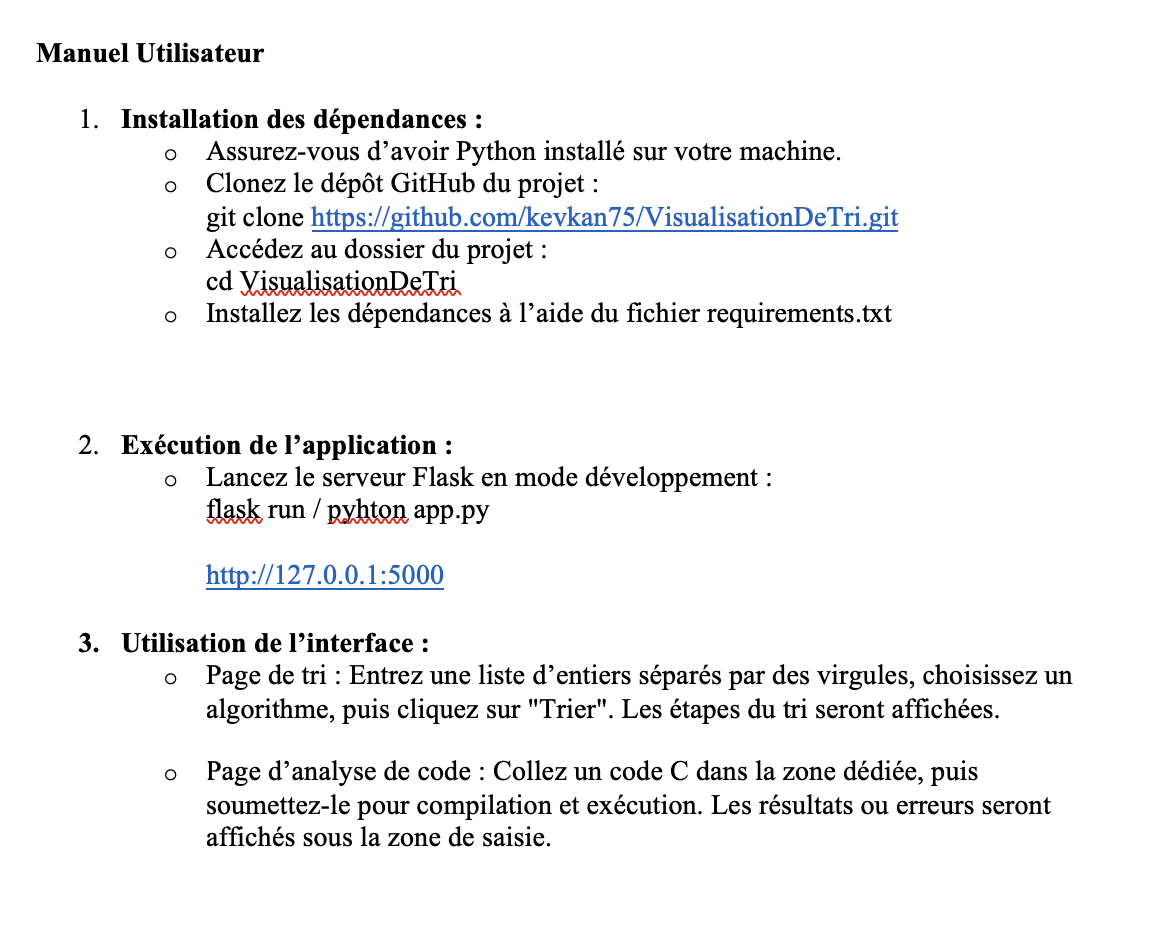
\includegraphics[width=\textwidth]{1.png}
    \caption{Manuel d'utilisateur}
    \label{fig:manuel1}
\end{figure}

\subsection{Page de tri}
\begin{figure}[H]
    \centering
    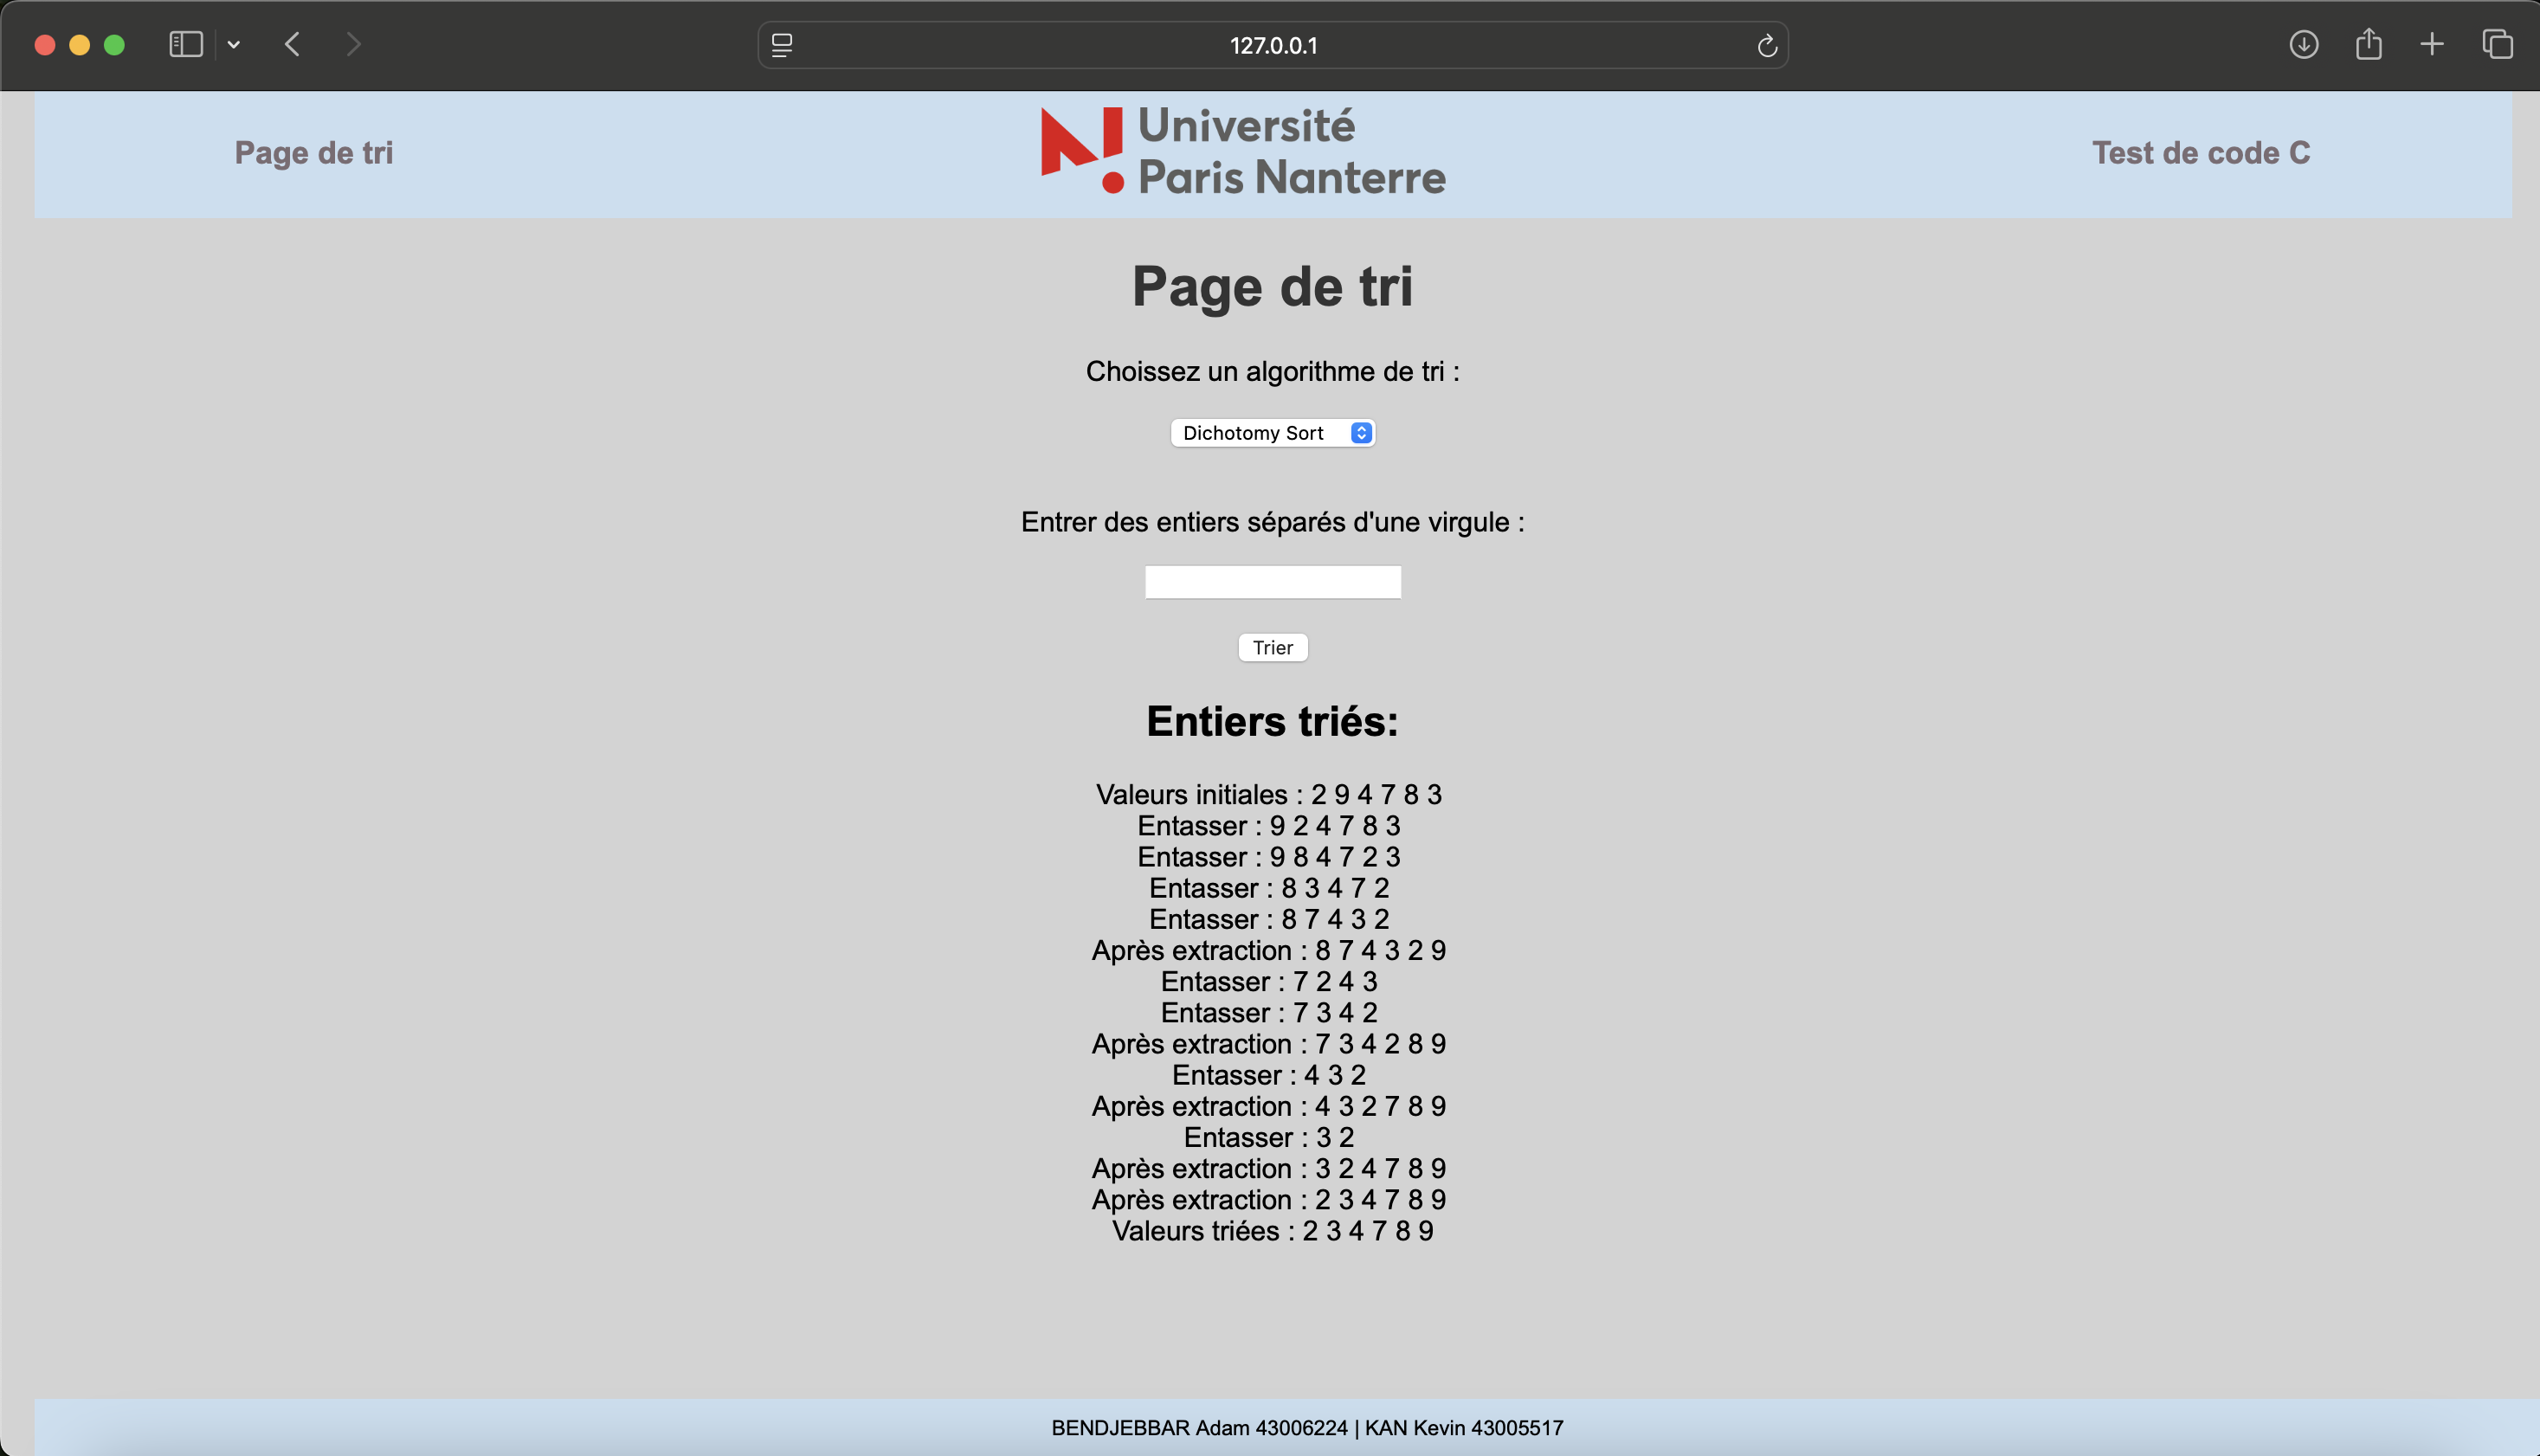
\includegraphics[width=\textwidth]{tri.png}
    \caption{Test de tri dichotomique}
    \label{fig:manuel2}
\end{figure}

\subsection{Page d'analyse de code}
\begin{figure}[H]
    \centering
    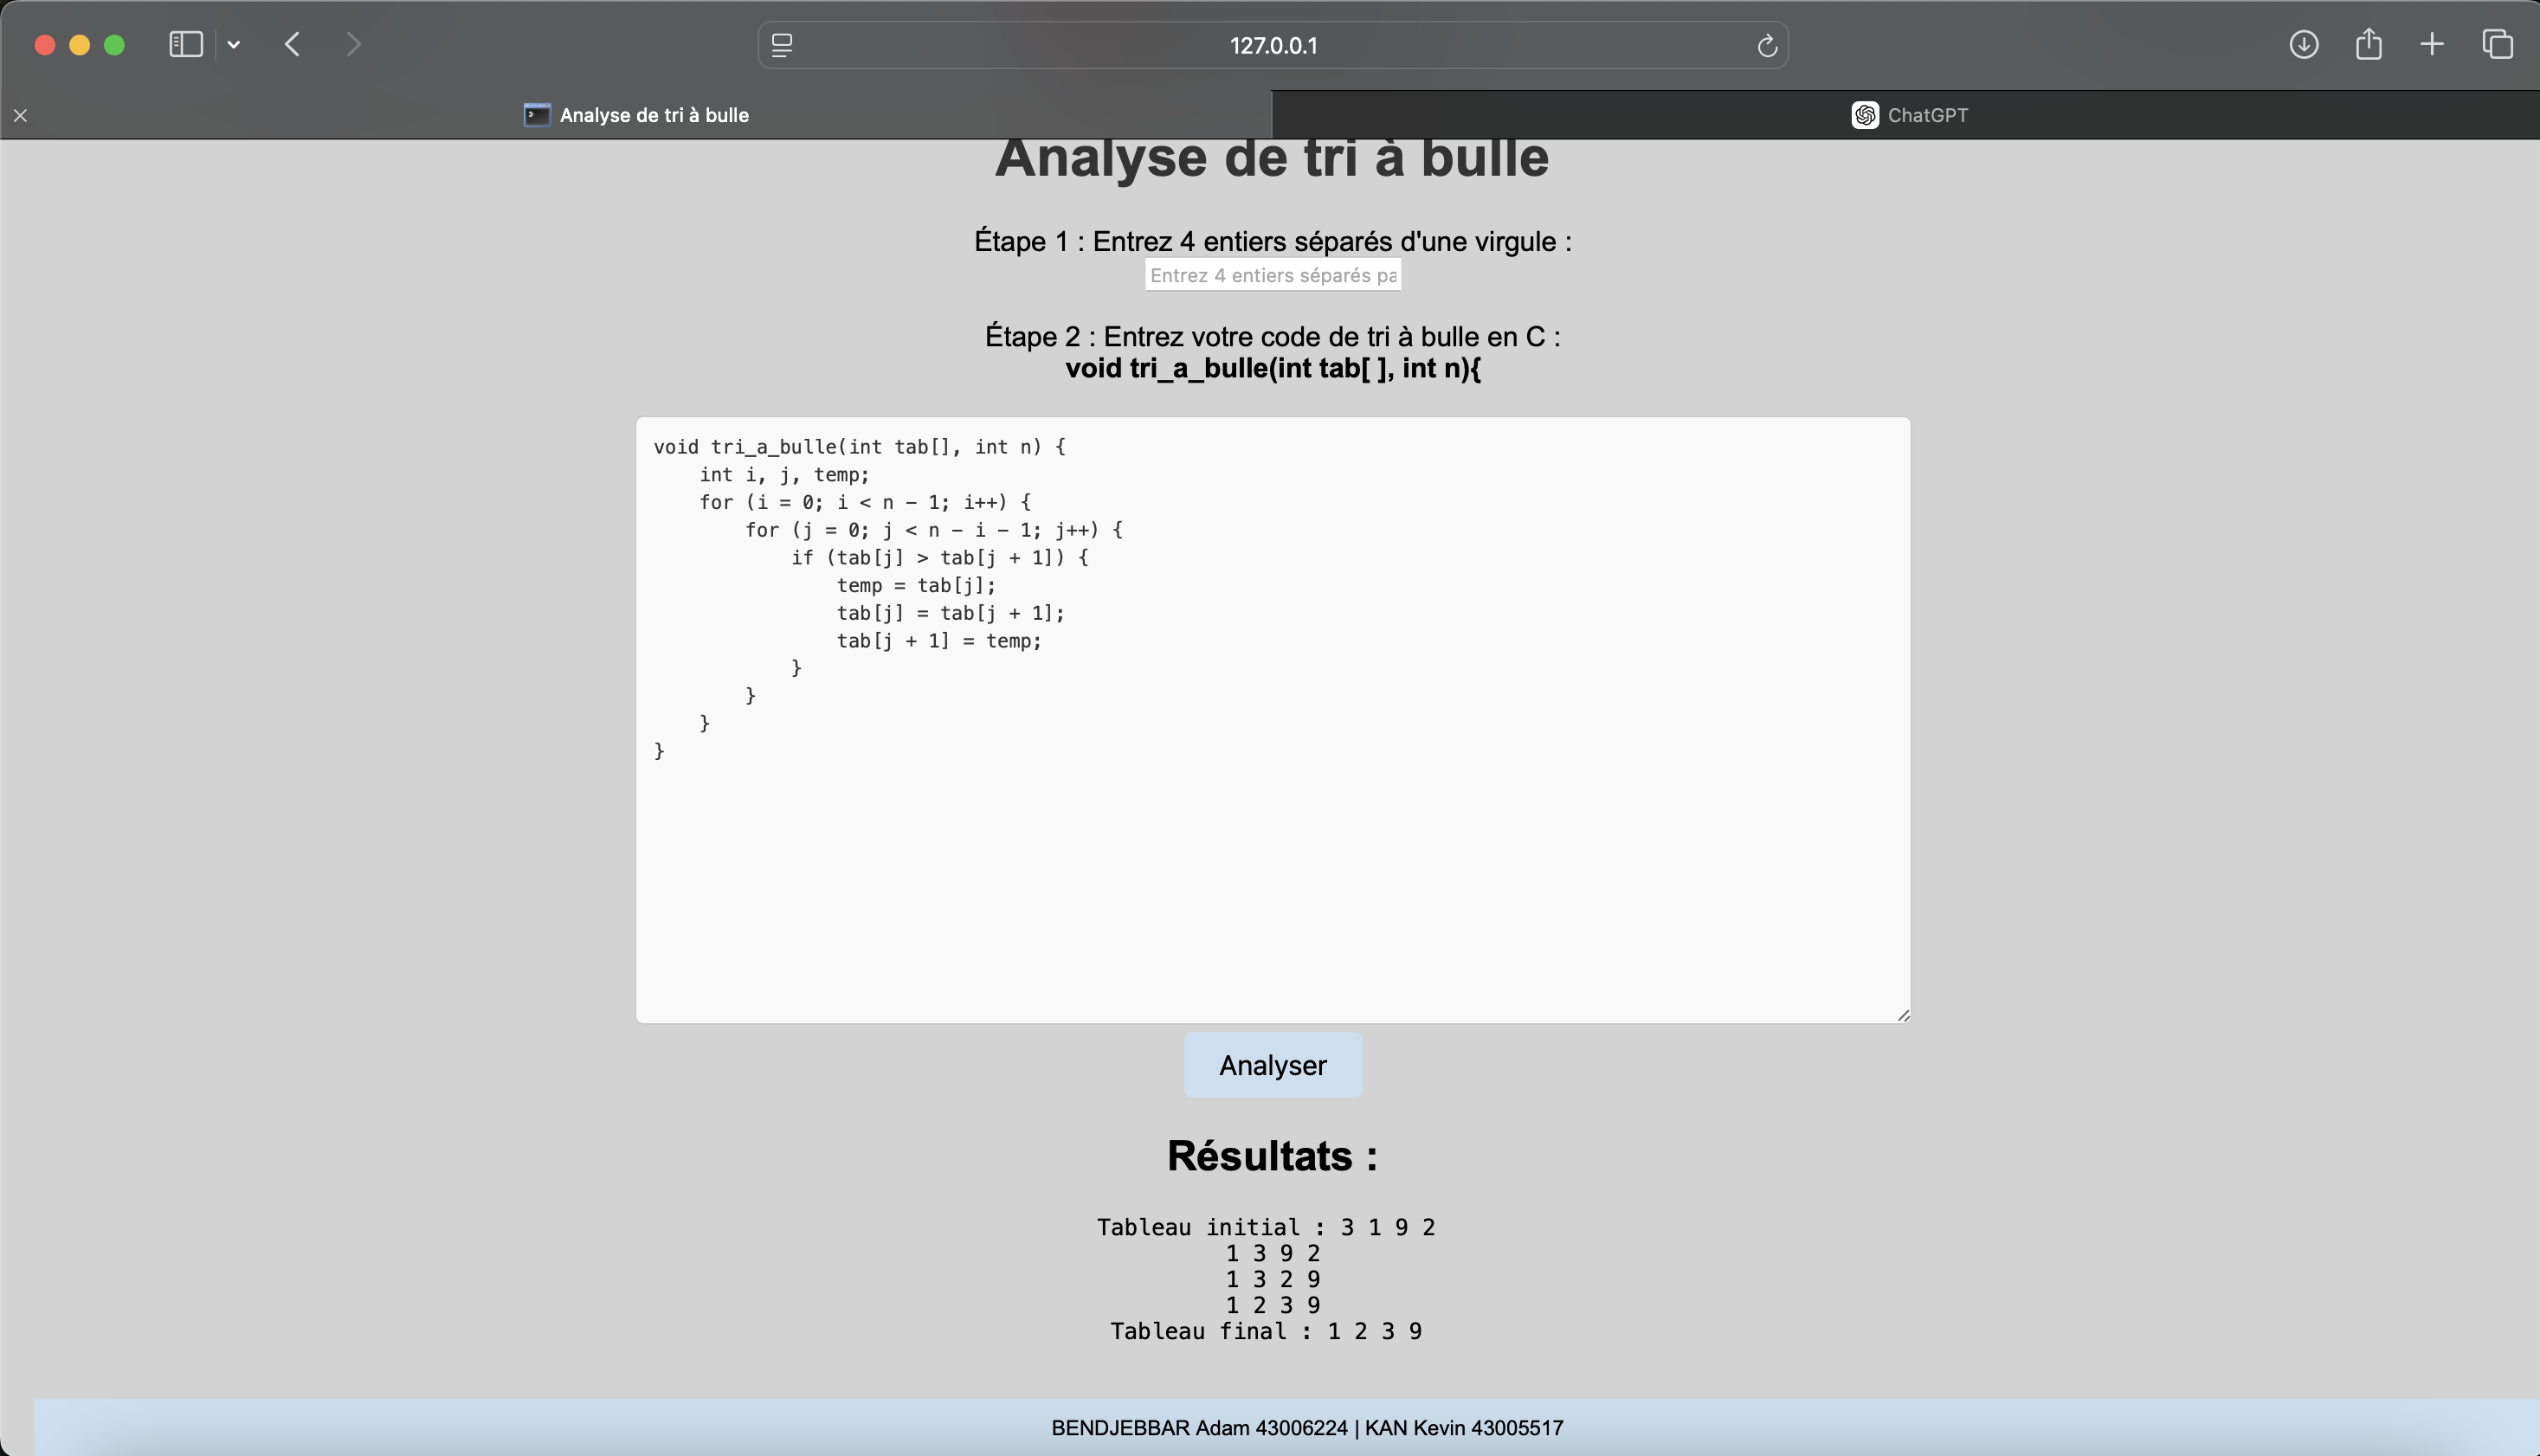
\includegraphics[width=\textwidth]{croissant.png}
    \caption{Test de tri à bulle croissant}
    \label{fig:manuel3}
\end{figure}
\begin{figure}[H]
    \centering
    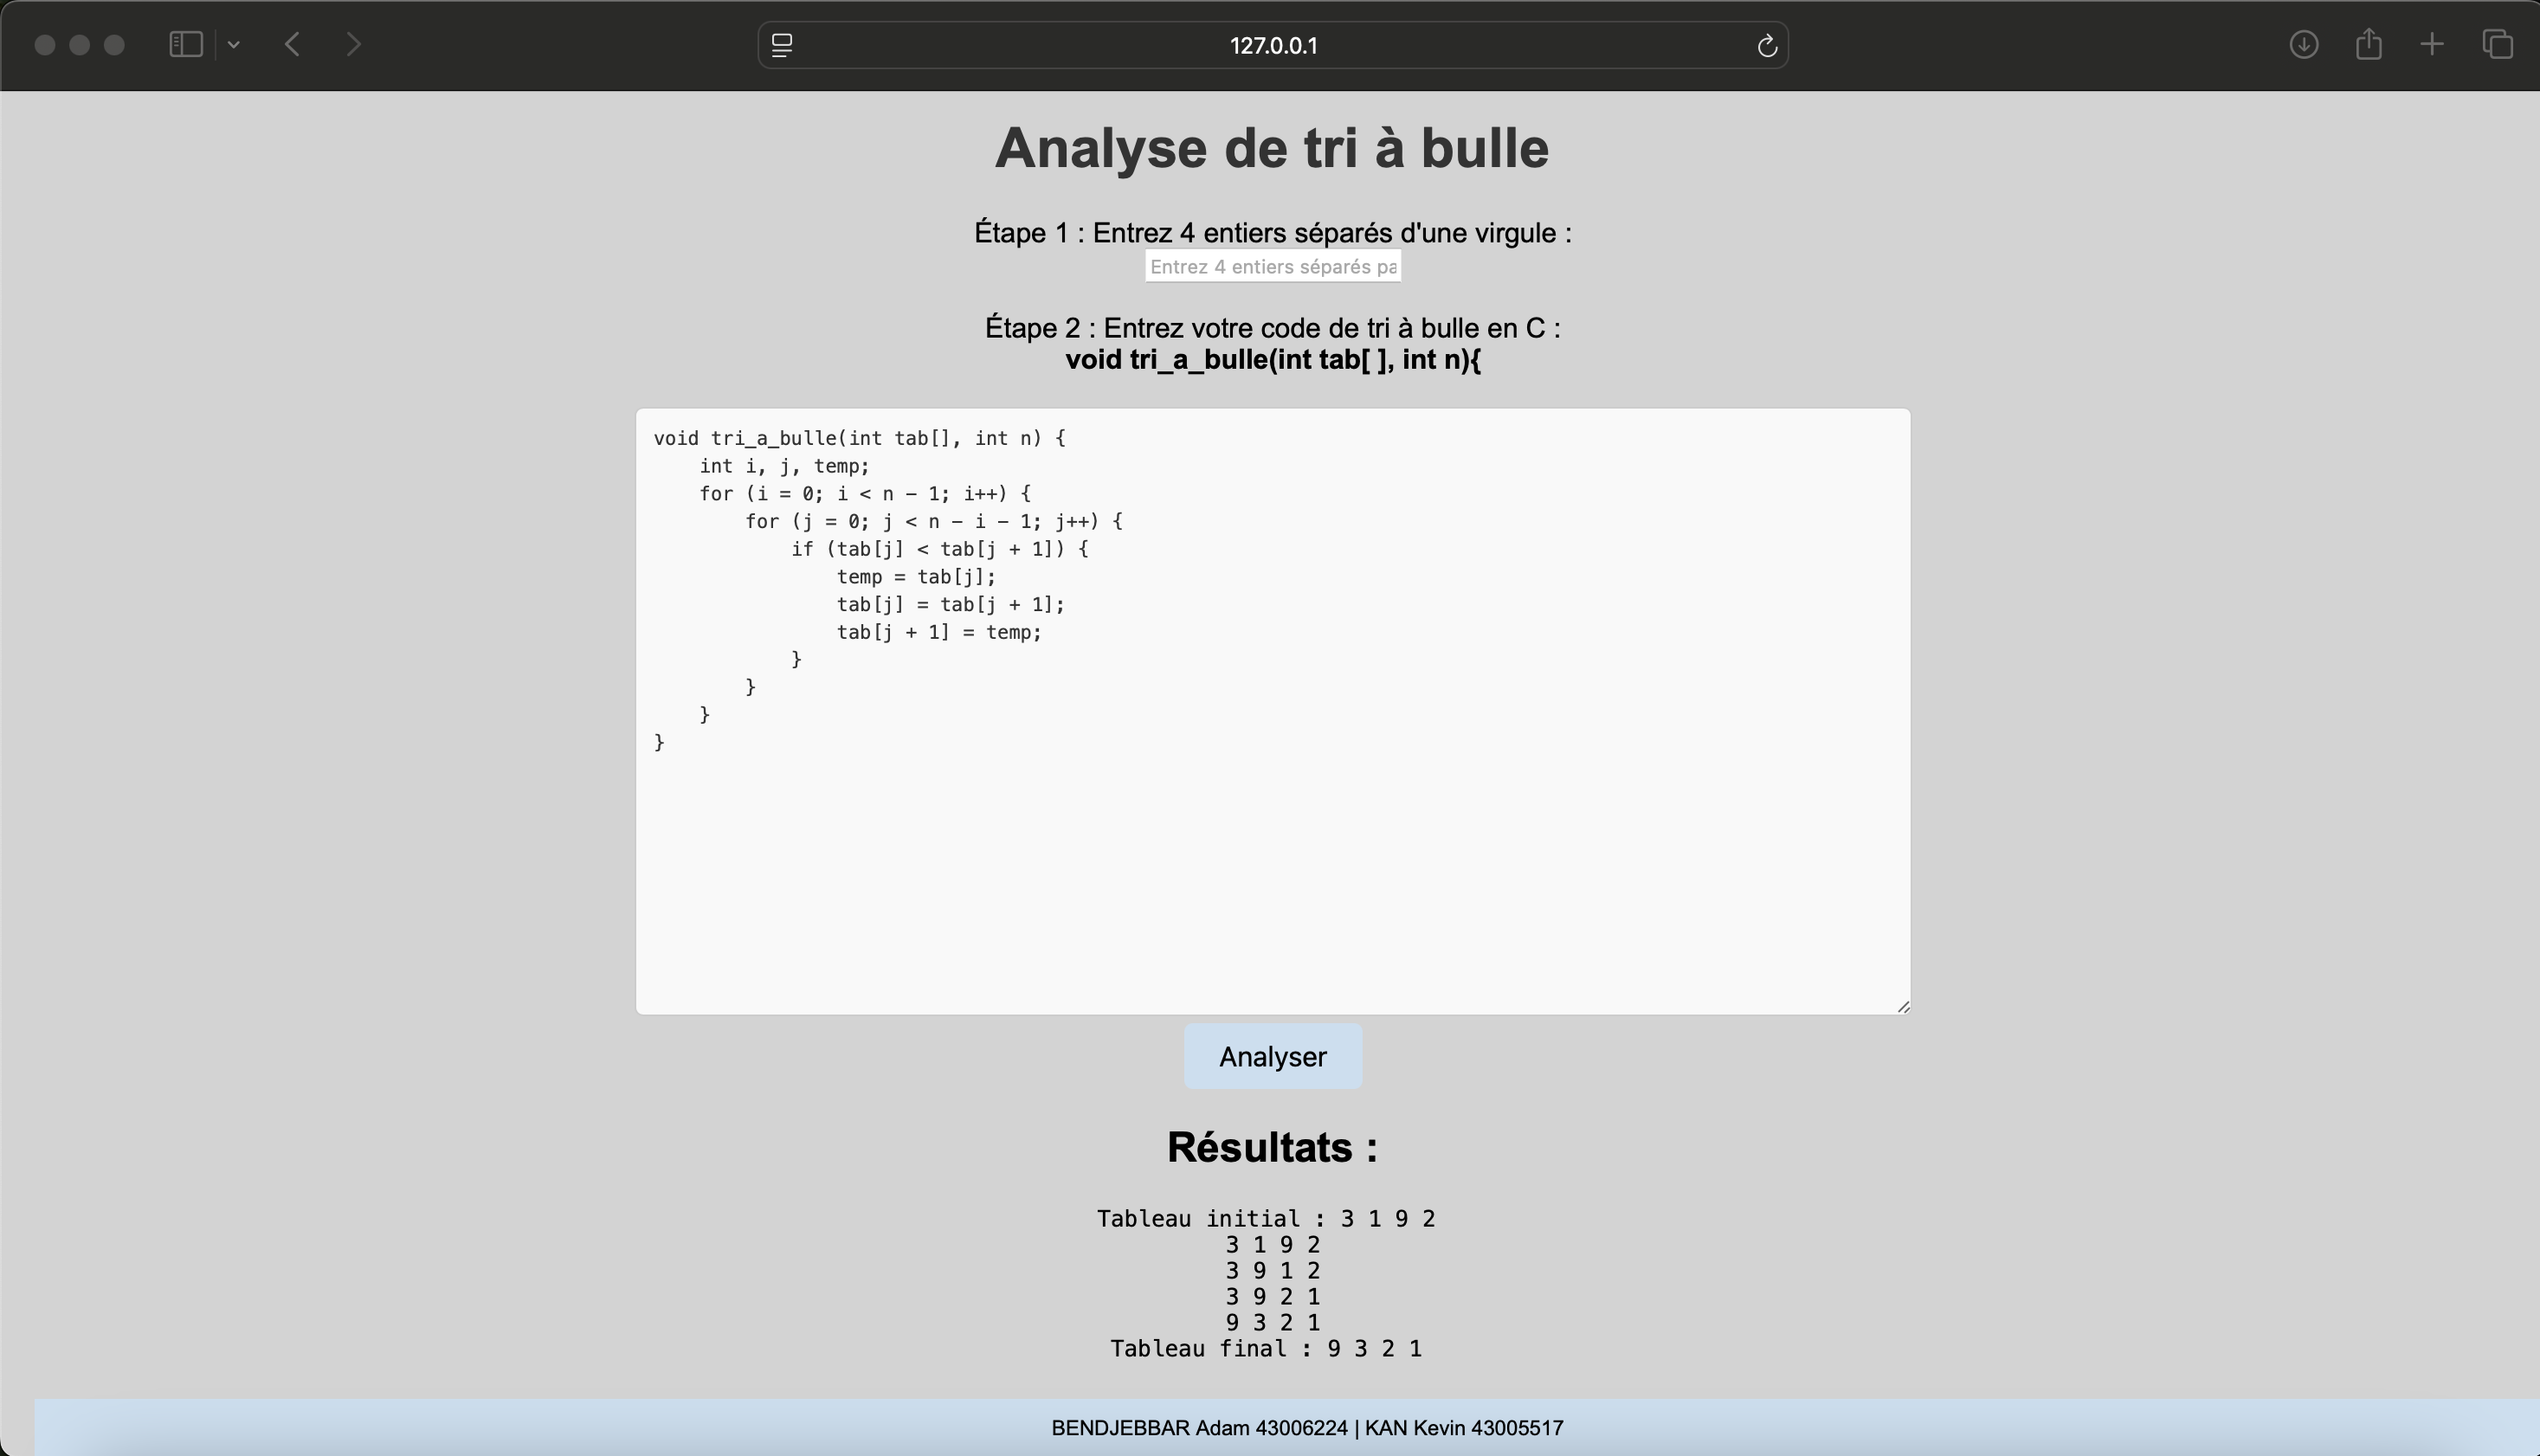
\includegraphics[width=\textwidth]{decroissant.png}
    \caption{Test de tri à bulle décroissant}
    \label{fig:manuel4}
\end{figure}
\begin{figure}[H]
    \centering
    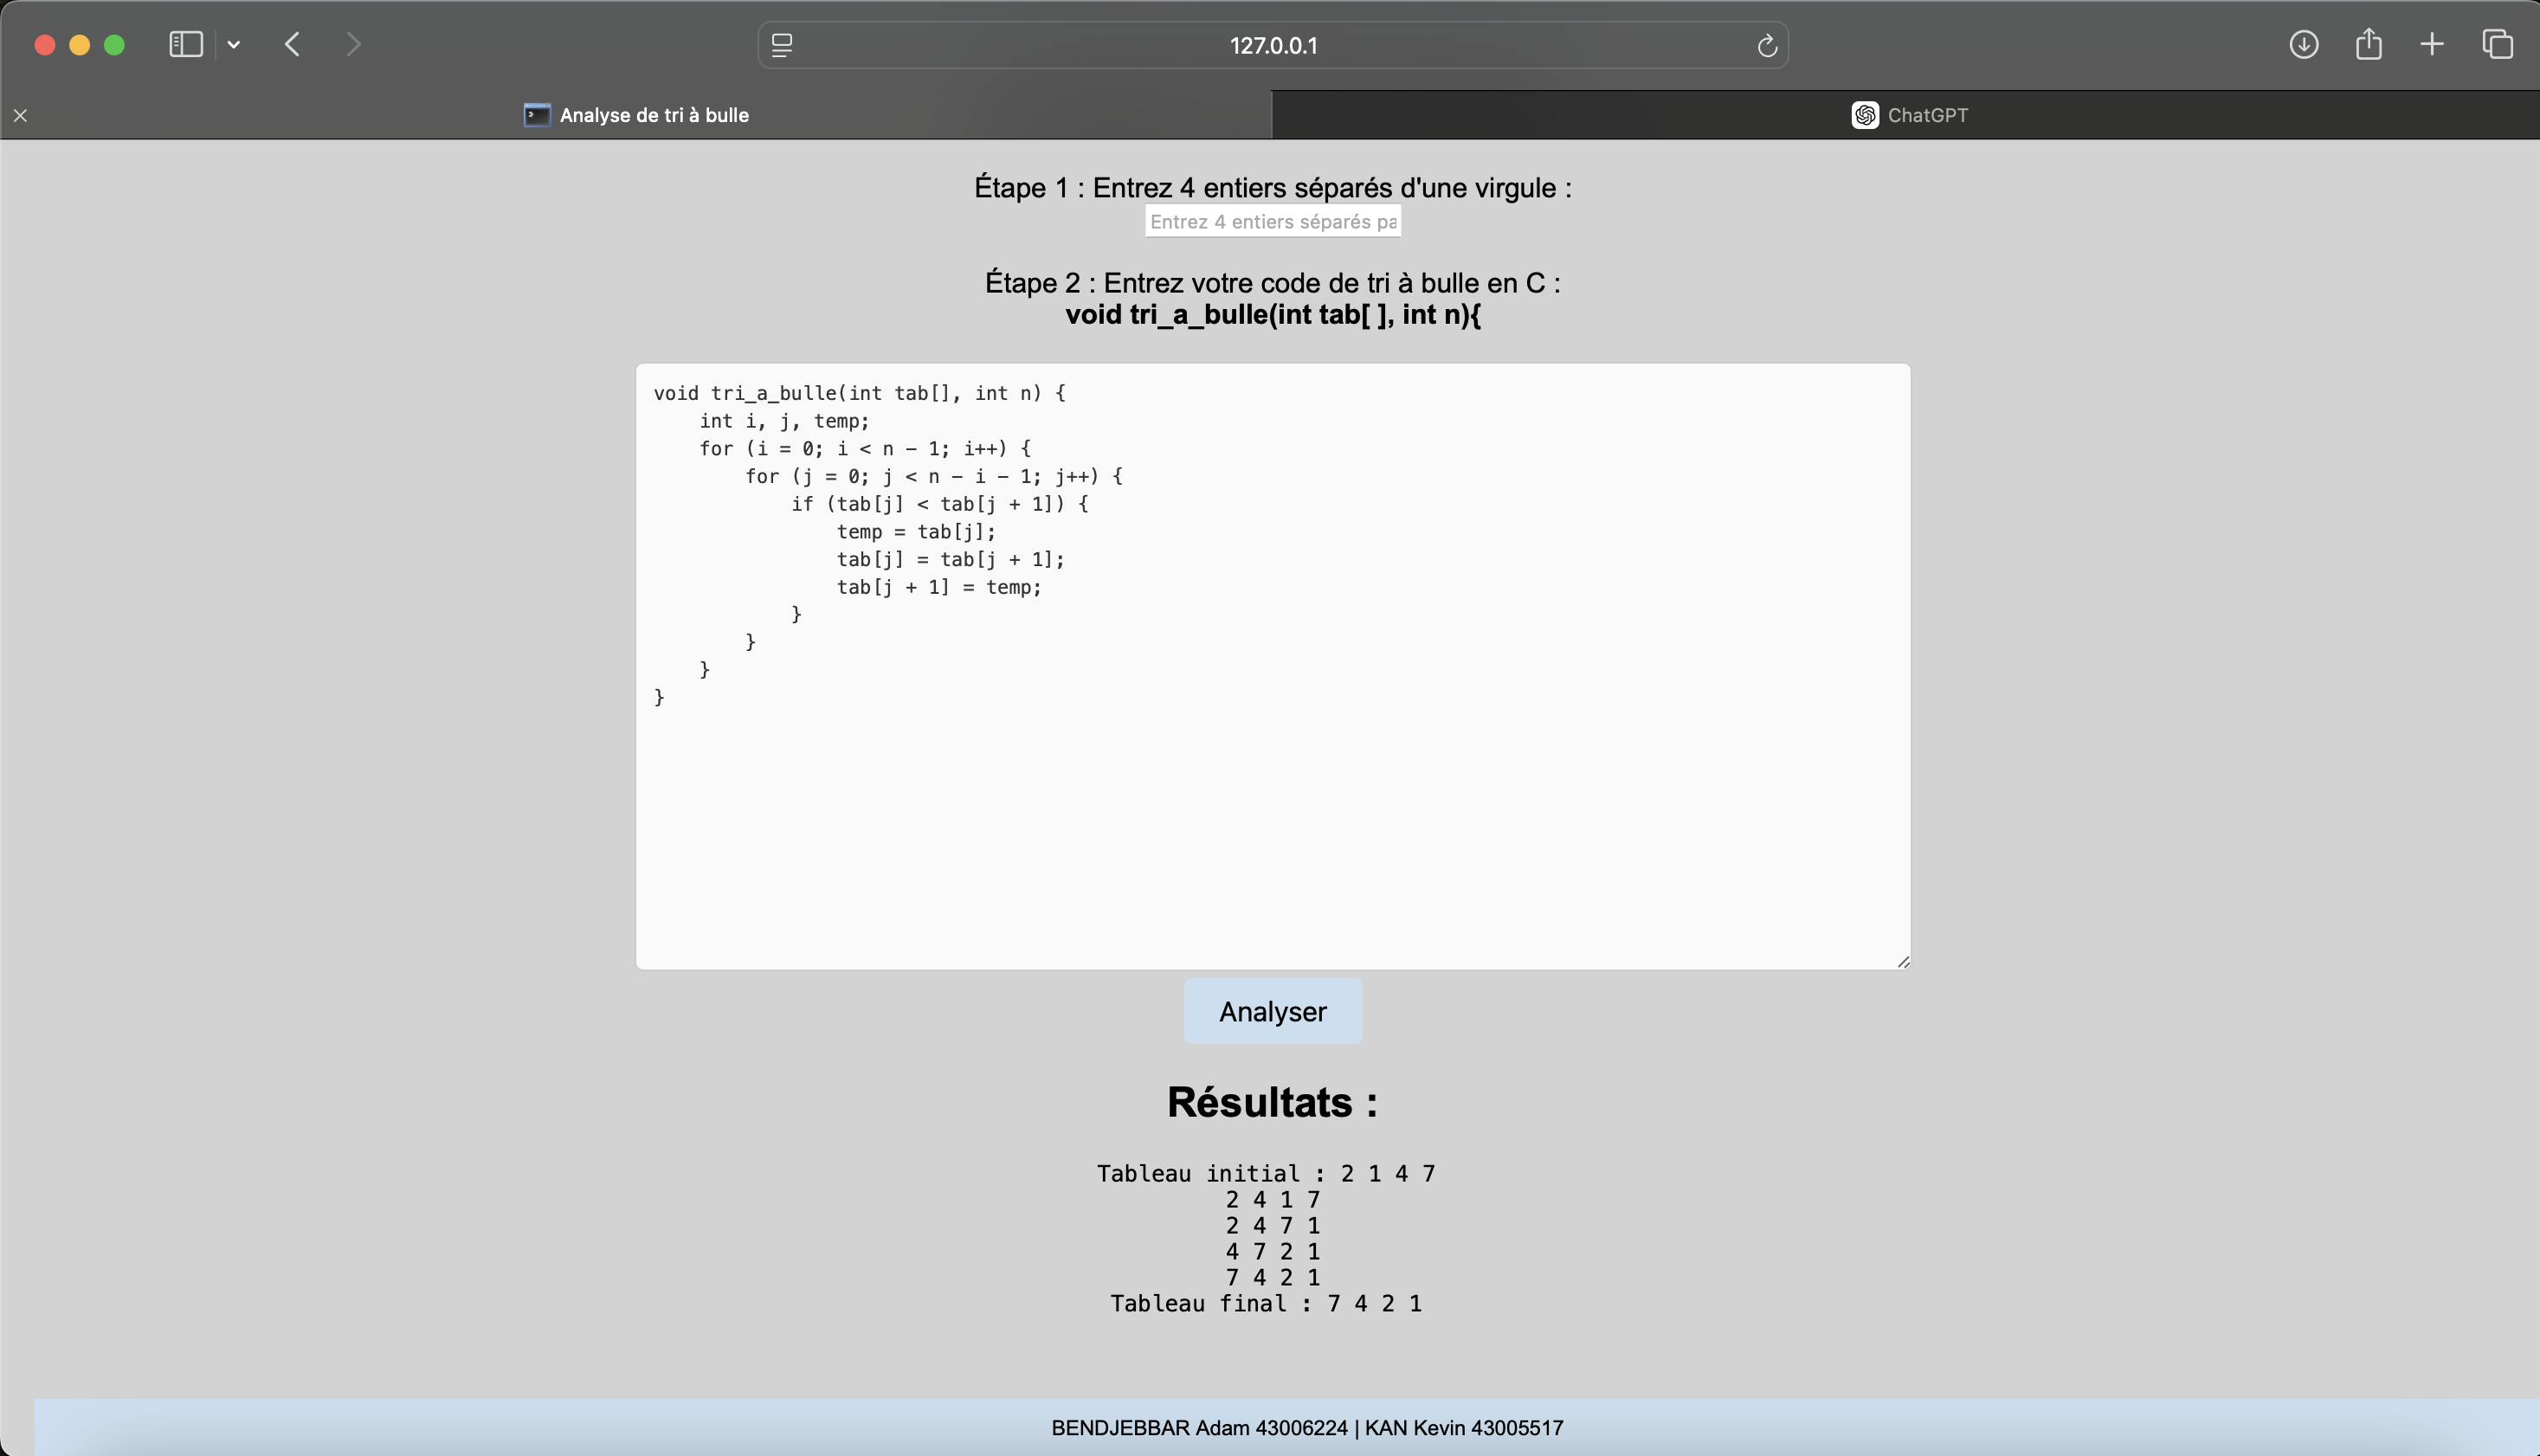
\includegraphics[width=\textwidth]{decroissant 2.png}
    \caption{Test de tri à bulle décroissant}
    \label{fig:manuel5}
\end{figure}


\end{document}
